% 3D periodic Fourier mode -- case_3d_mode.py.
% Triply-periodic cube, T = T0 + A sin(kx) sin(ky) sin(kz), k = 2 pi/L.
% Alternating hot/cold lobes (a 3D checkerboard) decay isotropically:
%   T0 + A sin sin sin * exp(-alpha * 3 k^2 t).
%
% Compile:  pdflatex setup_3d_mode.tex
\documentclass[border=6pt]{standalone}
\usepackage{amsmath}
\usepackage{tikz}
\usetikzlibrary{arrows.meta}

\definecolor{coldc}{RGB}{46,86,149}
\definecolor{hotc}{RGB}{171,57,52}
\definecolor{inkc}{RGB}{30,30,30}

\begin{document}
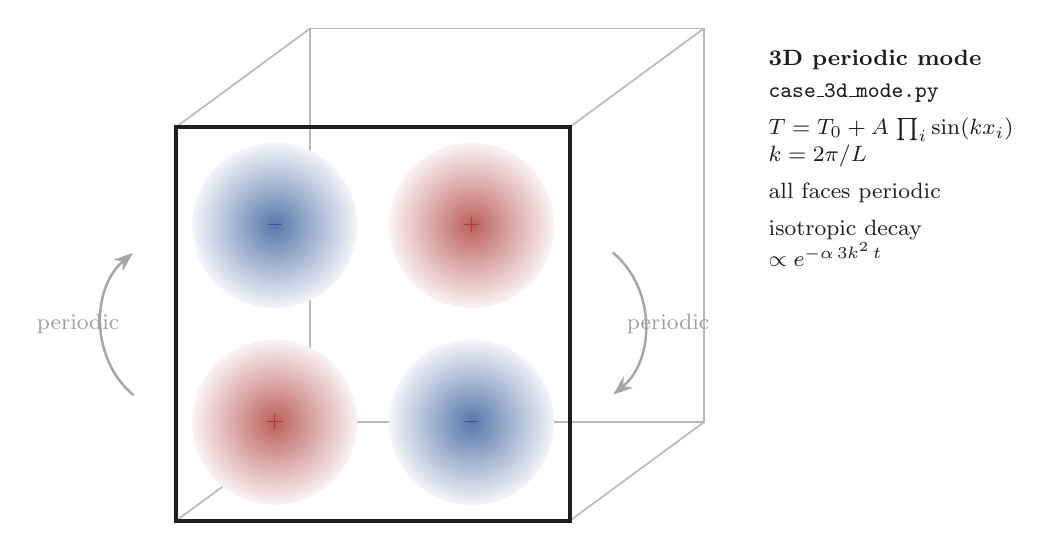
\begin{tikzpicture}[>=Stealth, font=\footnotesize, line cap=round]
  \def\S{5}        % front-face side
  \def\dx{1.7}     % oblique depth offset x
  \def\dy{1.25}    % oblique depth offset y

  % back face
  \draw[gray!55, line width=0.6pt]
    (\dx,\dy) -- (\S+\dx,\dy) -- (\S+\dx,\S+\dy) -- (\dx,\S+\dy) -- cycle;
  % connecting edges
  \draw[gray!55, line width=0.6pt] (0,0)--(\dx,\dy);
  \draw[gray!55, line width=0.6pt] (\S,0)--(\S+\dx,\dy);
  \draw[gray!55, line width=0.6pt] (\S,\S)--(\S+\dx,\S+\dy);
  \draw[gray!55, line width=0.6pt] (0,\S)--(\dx,\S+\dy);

  % 2x2 checkerboard of sin*sin lobes on the front face (pattern repeats in depth)
  \foreach \i/\j/\c in {0/0/hotc, 1/0/coldc, 0/1/coldc, 1/1/hotc}{
    \shade[inner color=\c!80, outer color=\c!6]
      ({1.25+2.5*\i},{1.25+2.5*\j}) circle (1.05);
  }
  \node[hotc,  font=\footnotesize\bfseries] at (1.25,1.25) {$+$};
  \node[coldc, font=\footnotesize\bfseries] at (3.75,1.25) {$-$};
  \node[coldc, font=\footnotesize\bfseries] at (1.25,3.75) {$-$};
  \node[hotc,  font=\footnotesize\bfseries] at (3.75,3.75) {$+$};

  % front face frame
  \draw[inkc, line width=1.4pt] (0,0) rectangle (\S,\S);

  % periodic-BC wrap arrows on opposite faces
  \draw[->, gray!70, line width=0.9pt] (-0.55,1.6) to[out=140,in=220] (-0.55,3.4);
  \draw[->, gray!70, line width=0.9pt] (\S+0.55,3.4) to[out=-40,in=40] (\S+0.55,1.6);
  \node[gray!75, anchor=east] at (-0.6,2.5) {periodic};
  \node[gray!75, anchor=west] at (\S+0.6,2.5) {periodic};

  % annotation
  \node[inkc, anchor=west, align=left] at (\S+\dx+0.7,\S-0.4)
    {\textbf{3D periodic mode}\\[2pt]
     \texttt{case\_3d\_mode.py}\\[4pt]
     $T=T_0+A\,\prod_i\sin(k x_i)$\\
     $k=2\pi/L$\\[4pt]
     all faces periodic\\[4pt]
     isotropic decay\\
     $\propto e^{-\alpha\,3k^2\,t}$};
\end{tikzpicture}
\end{document}
